\documentclass[11pt]{article}
\usepackage[a4paper,margin=0.86in]{geometry}
\usepackage{amsmath,amssymb,amsthm,mathtools}
\usepackage{graphicx}
\usepackage[hidelinks]{hyperref}
\usepackage{microtype}

\newtheorem{theorem}{Theorem}
\newtheorem{lemma}{Lemma}
\newcommand{\D}{\mathbb D}
\newcommand{\C}{\mathbb C}
\newcommand{\Hinfty}{H^\infty}

\title{The exponential moon is the missing winding-number counterexample}
\author{Full negative answer to an open question in arXiv:2406.07656}
\date{17 August 2026}

\begin{document}
\maketitle

\paragraph{Status.}
Candidate full counterexample, together with a sharp classification of all
symbols $e^{az}$. This is a new-result claim subject to human review.

\section*{Source question}

Gonz\'alez and Le\'on-Saavedra prove that constant winding number is necessary
for an entire symbol to induce an analytic Toeplitz operator with the double
commutant property. They ask whether it is sufficient, and specifically
suggest $\varphi(z)=e^{\pi i z}$ as a possible counterexample.

\begin{center}

\includegraphics[width=\textwidth]{figures/open_question_crop.png}
\end{center}

Here $M_\varphi$ denotes multiplication by $\varphi$ on $H^2(\D)$, and the
double commutant property is
\[
 \overline{\operatorname{Alg}(M_\varphi)}^{\mathrm{WOT}}
       =\{M_\varphi\}^{\prime\prime}.
\]

\section*{Main result}

\begin{theorem}\label{thm:main}
The entire function
\[
                         \varphi(z)=e^{\pi i z}
\]
has winding number one about every point of $\varphi(\D)$, but
$M_\varphi$ does not have the double commutant property. Consequently, the
winding-number condition in arXiv:2406.07656 is not sufficient.

More generally, for $a\in\C$,
\[
 M_{e^{az}}\text{ has the double commutant property}
 \quad\Longleftrightarrow\quad a=0\text{ or }|a|<\pi .
\]
\end{theorem}

\section*{Exact geometry of the critical image}

Let $\Omega=\varphi(\D)$. If $\varphi(z_1)=\varphi(z_2)$, then
$z_1-z_2=2k$ for some $k\in\mathbb Z$. Since two points of $\D$ have
distance strictly less than two, $\varphi$ is univalent on $\D$.

Write $w=re^{i\theta}$ with $-\pi<\theta<\pi$. The inverse branch is
\[
       z=\frac{\theta}{\pi}-\frac{i}{\pi}\log r,
\]
so
\begin{equation}\label{eq:image}
 \Omega=\left\{re^{i\theta}:
   -\pi<\theta<\pi,\quad \theta^2+(\log r)^2<\pi^2\right\}.
\end{equation}
Its boundary is the union of two Jordan loops
\[
 \Gamma_\pm:\qquad
 r=r_\pm(\theta):=
 \exp\!\left(\pm\sqrt{\pi^2-\theta^2}\right),
 \qquad -\pi\leq\theta\leq\pi .
\]
They meet only at $-1$ (the two endpoint arguments $\pm\pi$). Let $B$ be
the Jordan domain inside the outer loop $\Gamma_+$ and let $H$ be the
Jordan domain inside the inner loop $\Gamma_-$. Equation~\eqref{eq:image}
gives
\begin{equation}\label{eq:decomposition}
        \Omega=B\setminus\overline H,
        \qquad
        \overline H\cap\partial B=\{-1\}.
\end{equation}

\begin{center}
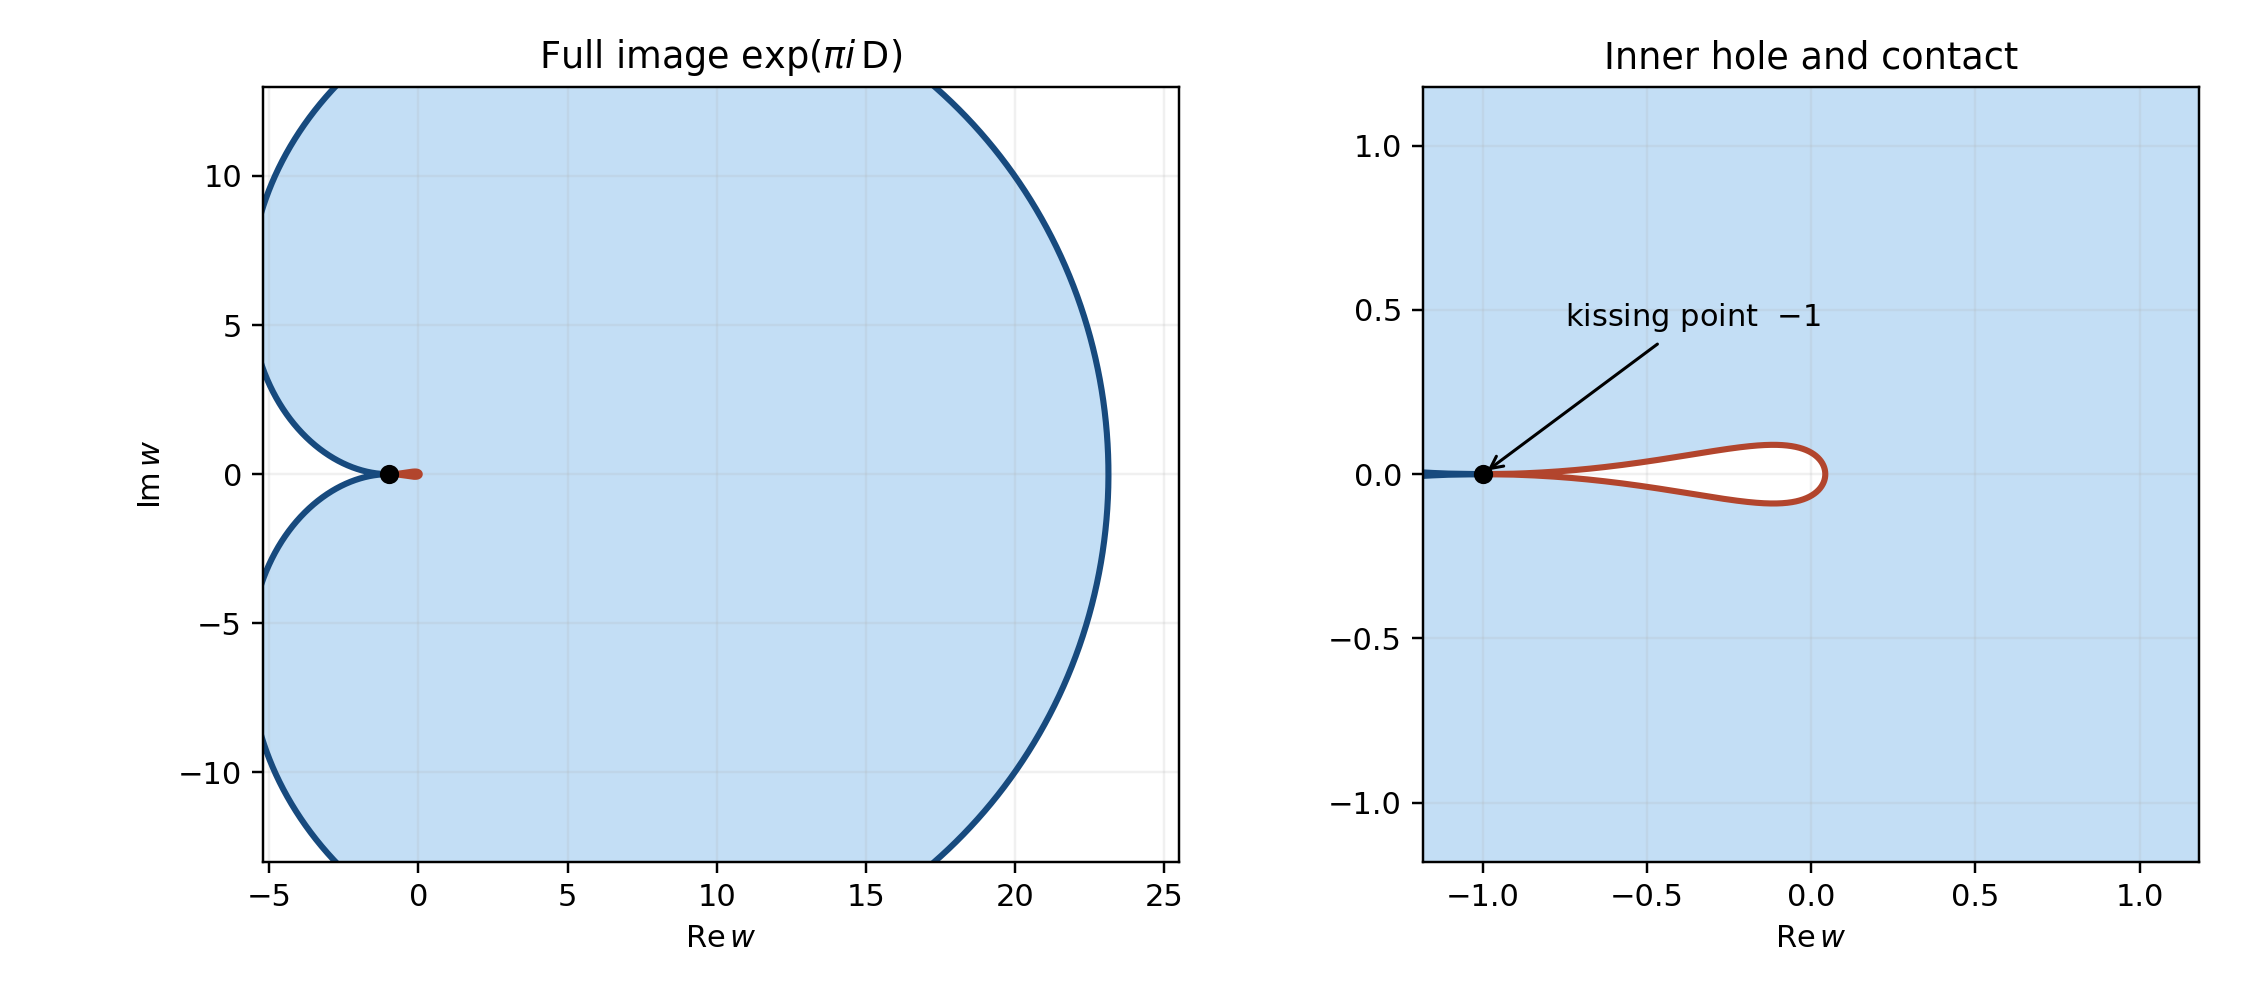
\includegraphics[width=0.86\textwidth]{figures/exponential_moon.png}
\end{center}

\section*{The relative-hull obstruction}

The subtlety is that failure of bounded polynomial approximation by a
single sequence does not by itself exclude weak-star generation: Sarason's
closure process may have transfinite order. The following argument uses his
full criterion.

Recall that a crosscut of a simply connected domain is a Jordan arc whose
open arc lies in the domain and whose two distinct endpoints lie on its
boundary. We claim that every crosscut of $B$ meets $\Omega$. Indeed, if a
crosscut $J$ missed $\Omega$, then by~\eqref{eq:decomposition}
\[
                   J^\circ\subseteq \overline H.
\]
Taking closures would put both endpoints of $J$ in
$\overline H\cap\partial B=\{-1\}$, contradicting their distinctness.

Sarason's Proposition~4 and its corollary now imply that the relative
$B$-hull of $\Omega$ is all of $B$. By the analytic definition of the
relative hull, every $f\in\Hinfty(B)$ satisfies
\begin{equation}\label{eq:norming}
                         \sup_B|f|=\sup_\Omega|f|.
\end{equation}
Since $B$ properly contains $\Omega$, Sarason's Corollary~2 says that a
Riemann map from $\D$ onto $\Omega$ is not a weak-star generator of
$\Hinfty(\D)$. Thus $\varphi$ is not a weak-star generator. Corollary~2.8
of the source paper states that for a univalent symbol, the double commutant
property is equivalent to weak-star generation. Hence $M_\varphi$ fails the
double commutant property.

On the other hand, $\varphi'$ never vanishes and every $c\in\Omega$ has
exactly one preimage in $\D$. No such $c$ lies on $\varphi(\partial\D)$.
The argument principle therefore gives
\[
                     n(\varphi(\partial\D),c)=1
                     \qquad(c\in\Omega).
\]
This proves the counterexample assertion.

\section*{Upgrade: the complete exponential phase transition}

Put $\varphi_a(z)=e^{az}$, $a\ne0$, and let
\[
                           p=\frac{2\pi i}{a}
\]
be a primitive period. If $|a|<\pi$, then $|p|>2$; hence $\varphi_a$ is
injective on $\overline\D$ and maps the circle to a Jordan curve. Walsh's
theorem gives weak-star density of the polynomials in $\varphi_a$, and the
source criterion gives the double commutant property.

If $|a|=\pi$, the rotation $z\mapsto (a/(\pi i))z$ reduces the image to
the critical moon above, so the property fails.

Finally suppose $|a|>\pi$, and put $s=|p|<2$. Choose a real-plane unit
vector $u\perp p$. Select
\[
                \sqrt{\max\{0,1-s^2\}}<r<1.
\]
The value $\varphi_a(ru)$ then has exactly one preimage in $\D$, because
all its preimages are $ru+kp$ and
$|ru+kp|^2=r^2+k^2s^2>1$ for $k\ne0$. In contrast, choose
\[
 0<\varepsilon<\sqrt{1-s^2/4}
\]
avoiding the finitely many values for which
$(k-\tfrac12)^2s^2+\varepsilon^2=1$ for some $k\in\mathbb Z$, and set
$q=-p/2+\varepsilon u$. Then
\[
 |q+kp|^2=(k-\tfrac12)^2s^2+\varepsilon^2.
\]
In particular, $q$ and $q+p$ lie in $\D$, while no translate lies on
$\partial\D$. Thus $\varphi_a(q)$ has at least two interior preimages and
is not on the boundary image. By the argument principle the winding number
is nonconstant, and
Theorem~5.9 of the source paper rules out the double commutant property.
For $a=0$, the operator is scalar and the property is immediate. This
completes the proof of Theorem~\ref{thm:main}. \qed

\section*{Verification and novelty}

The included script \texttt{code/verify\_exponential\_family.py} checks the
polar inverse formula on $20{,}000$ random disk points, checks the two
boundary arcs and the $|a|>\pi$ preimage witnesses, and numerically computes
winding number one for five interior test values using $200{,}001$ boundary
samples. It also generates the displayed figure. These checks support, but
are not used in place of, the exact proof.

A bounded novelty search covered the run indexes, the exact arXiv id,
searches combining $e^{\pi i z}$ with double commutants and weak-star
generation, and later citations visible in exact-title searches. No later
resolution was found. Novelty confidence is moderate, not exhaustive.

\section*{References}

\begin{enumerate}
\item M. J. Gonz\'alez and F. Le\'on-Saavedra,
\emph{Minimal commutant and double commutant property for analytic Toeplitz
operators}, arXiv:2406.07656; especially Corollary~2.8, Theorem~5.9, and
Section~6.
\item D. Sarason, \emph{Weak-star generators of $H^\infty$}, Pacific J.
Math. \textbf{17} (1966), 519--528; especially Proposition~4 and
Corollary~2 on pp.~525--527.
\end{enumerate}

\end{document}
